% \begin{figure}
%     \centering
%     \subcaptionbox{Velocity MSE\label{fig:results:mse_velocity}%
%     }[0.49\linewidth]{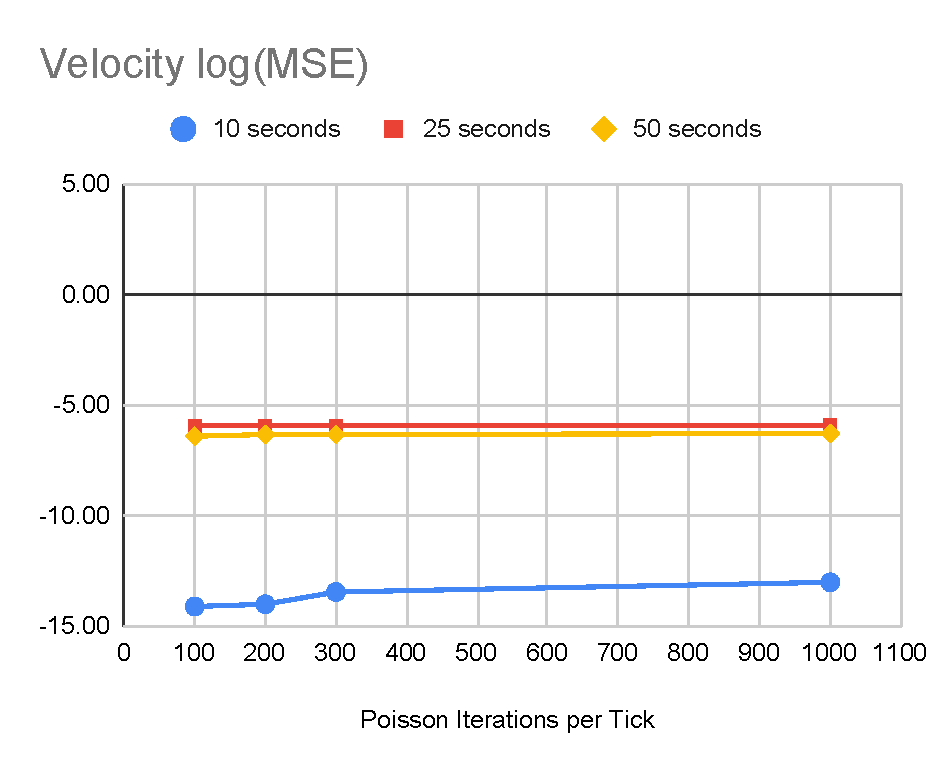
\includegraphics[width=\linewidth]{Ch62Results/figures/temp_velocity_mse.pdf}
%     }%
%     \subcaptionbox{Pressure MSE\label{fig:results:mse_pressure}%
%     }[0.49\linewidth]{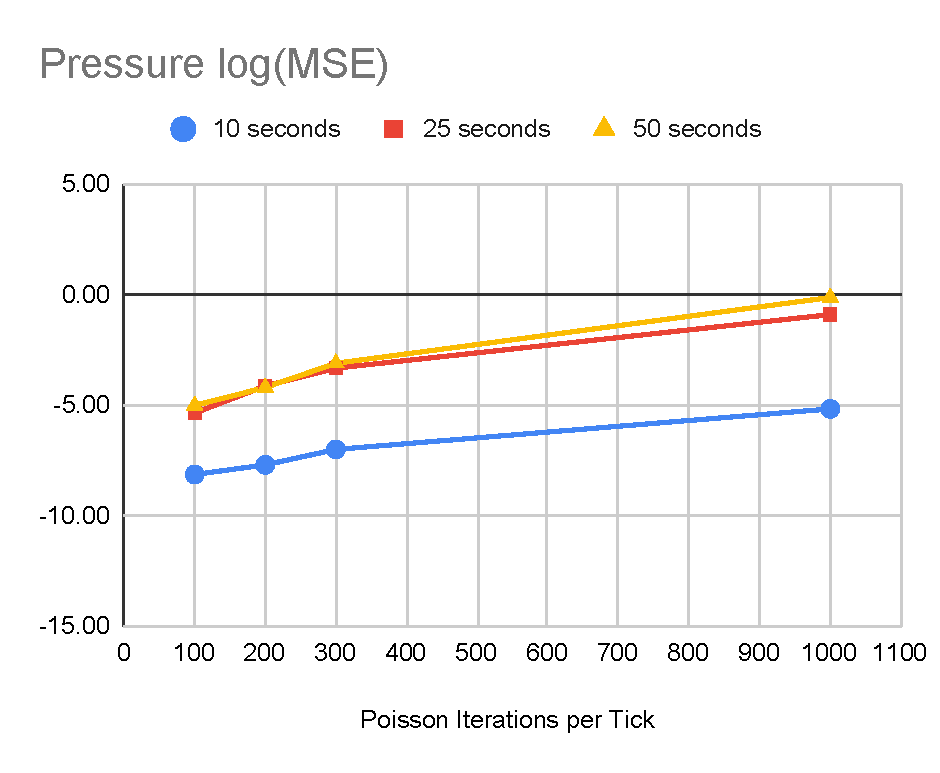
\includegraphics[width=\linewidth]{Ch62Results/figures/temp_pressure_mse.pdf}
%     }    
    
%     \caption{Initial MSE Results}
%     \label{fig:results:mse_initial}
% \end{figure}


\begin{figure}
    \centering
    \subcaptionbox{Velocity MSE\label{fig:results:mse_velocity}%
    }[0.49\linewidth]{
        \begin{tikzpicture}
        \begin{axis}[
            title={Velocity MSE},
            ylabel={MSE (log scale)},
            xlabel={Poisson Iterations per Tick},
            ymin=-15, ymax=5,
            xmin=0, xmax=1100,
            xtick={100,200,300,1000},
            ytick={5,0,-5,-10,-15},
            extra y ticks = {0},
            extra y tick labels = {},
            extra tick style = {
                grid=major,
                major grid style={line width=.5pt, draw=black}
            },
            yticklabels={$10^5$, $10^{0}$, $10^{-5}$, $10^{-10}$, $10^{-15}$},
            width=\linewidth,
        ]
        \addplot table [x=iters, y=vel-10, col sep=space] {Ch62Results/figures/data/MSE.csv};
        % \addlegendentry{\SI{10}{\second}};
        \addplot table [x=iters, y=vel-25, col sep=space] {Ch62Results/figures/data/MSE.csv};
        % \addlegendentry{\SI{25}{\second}};
        \addplot table [x=iters, y=vel-50, col sep=space] {Ch62Results/figures/data/MSE.csv};
        % \addlegendentry{\SI{50}{\second}};
        \end{axis}
        \end{tikzpicture}
    }%
    \subcaptionbox{Pressure MSE\label{fig:results:mse_pressure}%
    }[0.49\linewidth]{%
        \begin{tikzpicture}
        \begin{axis}[
            title={Pressure MSE},
            % ylabel={MSE (log scale)},
            xlabel={Poisson Iterations per Tick},
            ymin=-15, ymax=5,
            xmin=0, xmax=1100,
            xtick={100,200,300,1000},
            ytick={5,0,-5,-10,-15},
            extra y ticks = {0},
            extra y tick labels = {},
            extra tick style = {
                grid=major,
                major grid style={line width=.5pt, draw=black}
            },
            yticklabels={},%$10^5$, $10^{0}$, $10^{-5}$, $10^{-10}$, $10^{-15}$},
            legend pos=south east,
            width=\linewidth,
        ]
        \addplot table [x=iters, y=pres-10, col sep=space] {Ch62Results/figures/data/MSE.csv};
        \addlegendentry{\SI{10}{\second}};
        \addplot table [x=iters, y=pres-25, col sep=space] {Ch62Results/figures/data/MSE.csv};
        \addlegendentry{\SI{25}{\second}};
        \addplot table [x=iters, y=pres-50, col sep=space] {Ch62Results/figures/data/MSE.csv};
        \addlegendentry{\SI{50}{\second}};
        \end{axis}
        \end{tikzpicture}    
    }    
    
    \caption{Initial MSE Results}
    \label{fig:results:mse_initial}
\end{figure}